% !TeX root = Synopse.tex

\documentclass[12pt]{article}
\usepackage{lingmacros}
\usepackage{tree-dvips}
\usepackage[utf8]{inputenc}
\usepackage{fancyhdr}
\usepackage{listings}
\usepackage{subfig}
\usepackage{xcolor}
\usepackage{geometry}
\geometry{
a4paper,
total={170mm,257mm},
left=15mm,
top=20mm,
}
\usepackage{graphicx}
\usepackage{wrapfig}
\usepackage{amsmath}
\usepackage{hyperref}
\definecolor{link}{rgb}{0,0,215}
\hypersetup{
    colorlinks=true,
    linkcolor=link,
    filecolor=link,      
    urlcolor=link,
    pdfpagemode=FullScreen,
}

\graphicspath{ {./img} }

\definecolor{comment}{rgb}{0,0.45,0}
\definecolor{codegray}{rgb}{0.5,0.5,0.5}
\definecolor{codepurple}{rgb}{0.58,0,0.82}
\definecolor{backcolour}{rgb}{0.95,0.95,0.92}
\lstdefinestyle{CodeStyle}{
    backgroundcolor=\color{backcolour},   
    commentstyle=\color{comment},
    keywordstyle=\color{magenta},
    numberstyle=\tiny\color{codegray},
    stringstyle=\color{codepurple},
    basicstyle=\ttfamily\footnotesize,
    breakatwhitespace=false,         
    breaklines=true,                 
    captionpos=b,                    
    keepspaces=true,                 
    numbers=left,                    
    numbersep=5pt,                  
    showspaces=false,                
    showstringspaces=false,
    showtabs=false,                  
    tabsize=2
}
\lstset{style=CodeStyle}
\lstdefinelanguage{JavaScript}{
  keywords={typeof, new, true, false, catch, function, return, null, catch, switch, var, if, in, while, do, else, case, break},
  keywordstyle=\color{purple}\bfseries,
  ndkeywords={class, export, const, var, let, boolean, throw, implements, import, this, !!, !=, ===, ;},
  ndkeywordstyle=\color{blue}\bfseries,
  identifierstyle=\color{black},
  sensitive=false,
  comment=[l]{//},
  morecomment=[s]{/*}{*/},
  commentstyle=\color{comment}\ttfamily,
  stringstyle=\color{orange}\ttfamily,
  morestring=[b]',
  morestring=[b]"
}

%%%%%%% Document begin %%%%%%%%%%%
\begin{document}

\title{A* Algoritme}
\author{Johannes Jørgensen\\ S3o}
\date{2023 Febuar}
\maketitle

Projektets godkendelse og gennemgang af forløb.\\
Mit projekt (som er Pathfinding algoritmer) har jeg lavet lidt ændringer i mit gamle projekt, så den gamle kode er klar til at blive bygget videre på. Jeg vil gerne nå at implementere et vægtsystem i mit projekt, så min algoritmer kan blive lidt mere realistisk. Dette er til så min pathfinder skal kunne vurdere hvilken vej er nemmest og hurtigst vej fra A til B. Jeg er ikke begyndt endnu at implementere en ny algoritme (Jeg tænker A-star), da jeg først vil være klar med min gamle kode, samt have SOP overstået.  
Næste gang skal jeg også have lavet noget research inden for vægtet pathfinding, som jeg tænker er mit næste skridt i projektet. 
Efter det skal jeg implementere det og derefter gå videre med at implementere A-star algoritmen (måske nogle andre hvis jeg har tid)
Hvis jeg har meget tid til overs kan jeg gøre det visuelle mere lækkert at se på. 

\pagebreak
\tableofcontents
\pagebreak

%% Introduktion
\section{Resume}
Når du indtaster en destination ind på Google Maps på din telefon, hvordan finder Google Maps så den hurtigste vej? Kompleksiteten som Google Maps for at finde den hurtigste vej er umådelig stor, men en af elementerne som Google Maps bruger er Pathfinding Algoritmer. Formålet ved pathfinding algoritmer er at finde den korteste vej fra $a$ til $b$.
Jeg har i mit projekt opbygget et program som fremviser hvordan forskellige pathfinding algoritmer virker. Denne fremvisning er en visuel fremstilling af hvordan algoritmen påvirker et gitter miljø med forhindringer (vægge). Dette projekt bygger videre på mit tidligere projekt som jeg har lavet i 2.g hvor jeg havde en visuel fremstilling af Dijkstra’s algoritme. Men jeg har nu med et nyt design implementeret Astar (A*) algoritmen, som jeg vil have fokus på.

%% Teori
\section{Problemformulering}
Hvordan kan man med brug af Astar algoritme bruge ”Heuristics” til at finde den korteste vej fra $a$ til $b$ mest effektivt?
\section{Programbeskrivelse}
Mit program er en visuel fremvisning over hvordan pathfinding algoritmer fungerer og ”bevæger” sig i forhold til miljøet. Programmet er en webapplikation opbygget med et gitter af nogle celler, en ”Start” knap og forskellige indstillinger. 
Gitteren er hovedkomponentet i programmet, der er gitteret som er miljøet som pathfinding algoritmerne bevæger sig i. Miljøet kan brugeren selv ændre, med at placere og fjerne vægge som pathfinding algoritmerne ikke kan gå igennem. Dette gør det muligt for at brugeren kan eksperimentere med de forskellige algoritmer, samt udforske hvad algoritmerne vil gøre i forskellige situationer. Brugeren kan ændre forskellige indstiller som vil have effekt på hvordan algoritmen opføre sig. Disse forskellige indstillinger inkluderer størrelsen af gitteret (samt antallet af celler i gitteret), hastigheden på algoritmens køretid, Hvilken algoritme som skal køres og muligheden for at sætte tilfældige væge. 

\section{Teori}
A* (udtalt ”A-star”) eller Dijkstra er begge en algoritme i ”Pathfinding”, som er en computer applikation af den korteste vej mellem to punkter. Når der er tale om Pathfinding algoritmer og grafteori, skal vi først gennemgå forskellige relevante emner for at kunne bedre forstå problemet som pathfinding algoritmer løser. Her er det relevant at snakke om data-Trees, tidskompleksitet, Breadth-First Search (BFS) og Depth-first search (DFS). 
\subsection{Data-trees}
Data-trees inde for grafteori er en populær måde at bruge som en abstrakt form for data type, som repræsenterer et hierarkisk data-tree med forbundet ”celler” (”nodes” bliver brugt i samme sammenhæng). Hver cell er forbundet til en ”parent” cell, bortset fra start cellen eller roden af data-treet, som ingen parent cell har. Disse begrænsninger betyder, at der ikke er nogen cyklusser og at hvert ”child” cell kan behandles som roden af sit eget ”subtree” (et indsnævret  mængde af celler i et større data-tree). Disse elementer gør at rekursion kan bruges som en brugbar teknik inden for data-trees.\\
\begin{figure}[ht]%
  \centering
  \subfloat[\centering Struktur for et data-tree]{{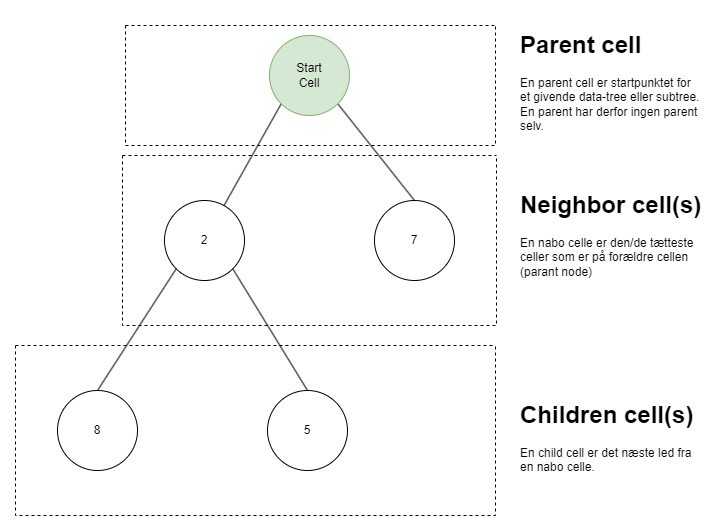
\includegraphics[width=0.7\textwidth]{../datatree.png} }}%
  \label{fig:datatree}%
\end{figure}
Der er flere forskellige metoder som bruges for at finde den korteste vej i et stort netværk af punkter og parameter. De to mest velkendte algoritmer er Breadth-First Search (BFS) og Depth-first search (DFS). 
Breadth-First Search algoritme søger de tætteste naboer før algoritmen går videre til det næste led af data celles i data-tree. Dette gør algoritmen uden forhold til nogle parametre eller ekstra viden om netværket den søger igennem. Depth-first search gør det omvendte af BFS, her søger DFS algoritmen først gennem en enkel gren før den gør tilbage til start cellen og gør det samme med en anden gren i data-tree. 

\subsection{Dijkstra’s algoritme}
Dijkstra’s algoritme er en variation af Breadth-First Search, men hvor Dijkstra’s algoritme gør brug af en prioriterings kø, som afgør hvilken nabo Dijkstra skal søge igennem først. 
Dijkstra starter med at angive en arbitrær afstandsværdi til alle celler i netværket: start cellen får afstandsværdien 0, hvor alle andre får afstandsværdien Infinity. 
Vores prioteringskø holder vi øje med alle undersøgte celler. For den nuværende celle, bliver alle naboer som ikke er undersøgt med (afstanden til nuværende celle) + (afstanden fra nuværende celle til naboen). Hvis denne afstandsværdi er mindre end den forrige arbitrær afstandsværdi, bliver den nye afstand værdi kun relevant. Når vi er færdige med at undersøge afstandsværdien for alle naboer, markere vi den nuværende celle som undersøgt.  

\subsection{A* algoritme}
A-star algoritmen er en videreudvikling af Dijkstra’s algoritme. Denne forlængelse er ved brug af målrettet heuristik, 
som gør det muligt for A-star at vide hvilke ruter som skal søges igennem først. 
Heuristik gør derfor A-star til en informeret søgealgoritme, eller en best-first search algoritme. 
Ved hver iteration af A-stars loop, skal algoritmen tag stilling til hvilken rute som skal søges. Dette gøres den baseret på omkostningerne af den rute, samt rutes estimeret omkostning som skal til for at bruge den rute hele vejen til slut. A-star brugere tre forskellige værdier til at beslutte dette: 
(hvor $n$ er den næste celle på den på givende rute)\\
\[g(n)\]
$g(n)$  er omkostningerne af ruten fra start til $n$.
\[h(n)\] 
$h(n)$ er den heuristiske værdi som estimerer omkostningerne af den billigste rute fra celle n til slut. 
Der er flere forskellige måder at beregne h værdien, enten beregne det præcise værdi for $h$ (dette kan kræve meget tid) eller en estimeret værdi for $h$ som tag mindre tid. En af disse måder kunne være med \textit{Manhattan Distance.} 
Manhattan Distance er summen af absolutte værdier af forskellen af henholdsvis X- og Y-koordinater mellem start og slut cellen. 
\begin{lstlisting}[language=JavaScript, caption=Manhattan Distance\label{code:Manhattan}]
  h = abs(current_cell.x - goal.x) + 
  abs(current_cell.y - goal.y)
\end{lstlisting}
\begin{figure}[ht]\label{fig:Manhattan}
  \centering
  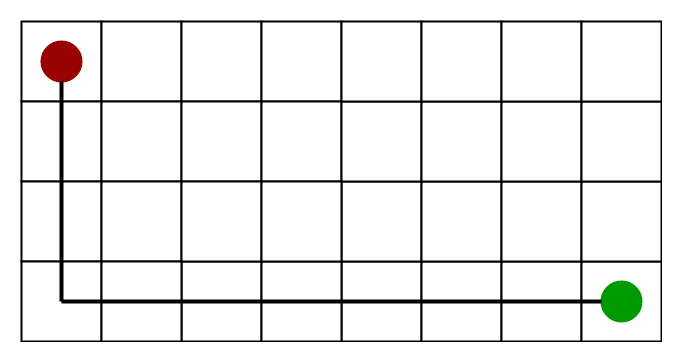
\includegraphics[width=0.50\textwidth]{../manhattan.png}
  \caption{Manhattan Distance Heuristics, med forskellen mellem x og y-koordinaterne (Evt. antag at rød plet er start cellen og grøn er slut cellen)}
\end{figure}
Efter beregningerne af $g(n)$ og $h(n)$, beregner vi den tredje værdi $f(n)$, 
som repræsenterer vores nuværende bedste gæt til den billigste vej fra start til slut:
\[f(n)= g(n) + h(n)\]

\section{Funktionalitet}
Det er vigtigt at når brugeren åbnet programmet, at de ikke er i tvivl om hvad der foregår. For at kunne opnå en høj funktionalitet opstiller jeg nogle krav. Dette inkluderer hvordan man køre algoritmen, vælger hastighed, gitter størrelse og sætte vægge. Samtidig skal det være intuitivt at se hvad der forgår, selvom man ikke forstår pathfinding. 
\begin{itemize}
  \item Brugeren skal kunne klikke på enkle punkter på gitteret for at kunne tilføje eller fjerne en væg, samt kunne nemt forstå at en væg er blevet fjernet eller tilføjet. 
  \item Det skal samtidig være simpelt at kunne ændre på nogle indstillinger for f.eks. hvor hurtig algoritmen køre eller hvor stort et gitter man vil bruge. 
  \item Når brugeren kører programmet, skal det være intuitivt at kunne forstå hvordan algoritmen fungere og hvilken vej som er den korteste fra $a$ til $b$.
\end{itemize}
\section{Brugergrænseflade}
Når et it-produkt bliver produceret og designet, er det vigtigt at brugeren af programmet kan anvende det uden irritation eller følelsen af utilstrækkelighed. Man designer derfor en brugergrænseflade som fokuserer på at gøre it-produktet tilfredsstillende for brugeren.
En brugergrænseflade er en form for bindeled mellem en bruger og et it-produkt eller system. Brugergrænsefladen modtager forskellige typer af inputs fra bruger, såsom klik med musen eller via tastaturet osv. Det input giver derefter et output og måske en form for feedback til brugeren, efter brugeren har interageret med it-produktet. 
\begin{table}[ht]
  {\renewcommand{\arraystretch}{1.2} %<- modify value to suit your needs
  \begin{tabular}{ |c|c| }
   \hline
   \textbf{Input fra brugeren} & \textbf{Output} \\ 
   \hline
   Klik på celle i gitter & \shortstack{Tilføj eller fjern væg i forhold \\ til om der allerede er en væg eller ej.} \\
   \hline
   ’Drag’ skyder under ”Animation Speed” & \shortstack{Ændre hastigheden for \\ animationen for algoritmen i ms.} \\
   \hline
   Klik på ”Start” knappen & Starter programmet med valgt algoritme. \\
   \hline
   \shortstack{Klik på en af ”Cell Size” knapperne \\(Big, Default, Small)} & Ændre Størrelsen på cellerne i gitteret. \\
   \hline
   Klik på en af algoritmeknapperne (Dijkstra eller Astar) & \shortstack{Ændre valget algoritme som bliver \\kørt når ”Start” knappen bliver trykket.} \\
   \hline
   Klik på ”random walls” knappen & \shortstack{Placere tilfældige væge i gitteret \\ som algoritmerne ikke må gå igennem.} \\
   \hline
  \end{tabular}}
\end{table}
\section{Diagrammer}
\subsection{UML-diagram}
\subsection{A* algoritme}


\section{Pseudokode}
\section{Udvalgt Kode}
\section{Konklusion}
\section{Bilag}

% https://i.gyazo.com/0b387356445aefc069204298e796aff7.mp4 
\end{document}